\paragraph{Soggetto 1}~

Per verificare le prestazioni e il funzionamento dei moduli progettati, sono state effettuate alcune misurazioni su un soggetto maschio, di età 55 anni, di carnagione chiara. Il soggetto si trovava in condizioni di riposo.

\paragraph{MAX86916}~

Di seguito sono riportati i risultati ottenuti utilizzando il sensore MAX86916.

\paragraph{Polpastrello indice sinistro}
\begin{figure}[h]
	\centering
	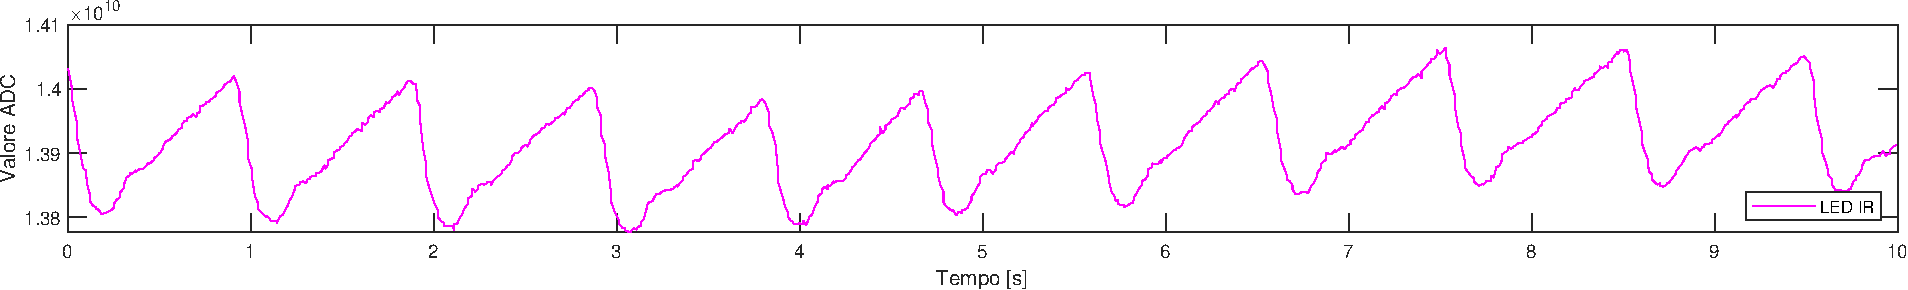
\includegraphics[width=1\linewidth]{ImageFiles/Misure Preliminari/Soggetto 1/polpastrello_ired}
	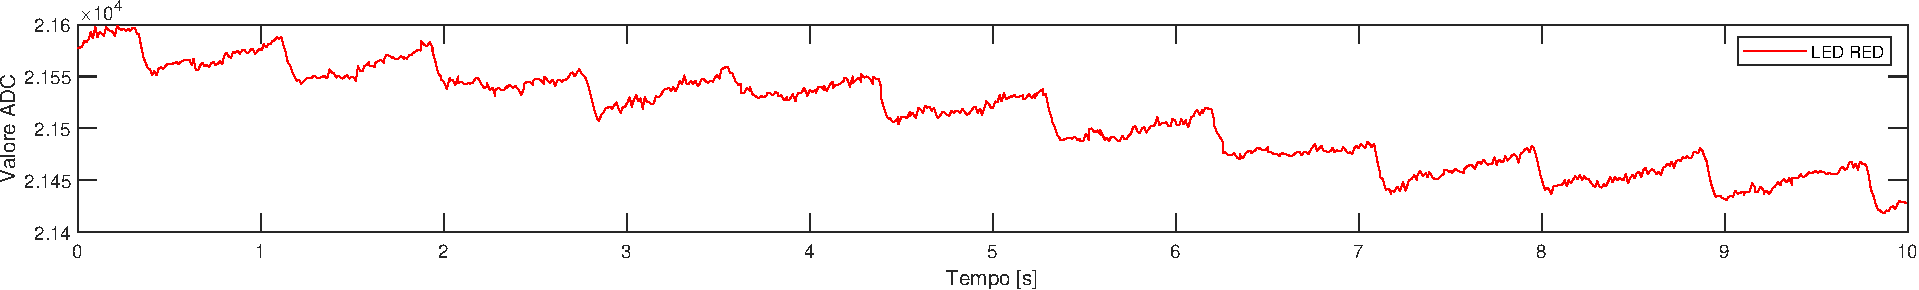
\includegraphics[width=1\linewidth]{ImageFiles/Misure Preliminari/Soggetto 1/polpastrello_red}
	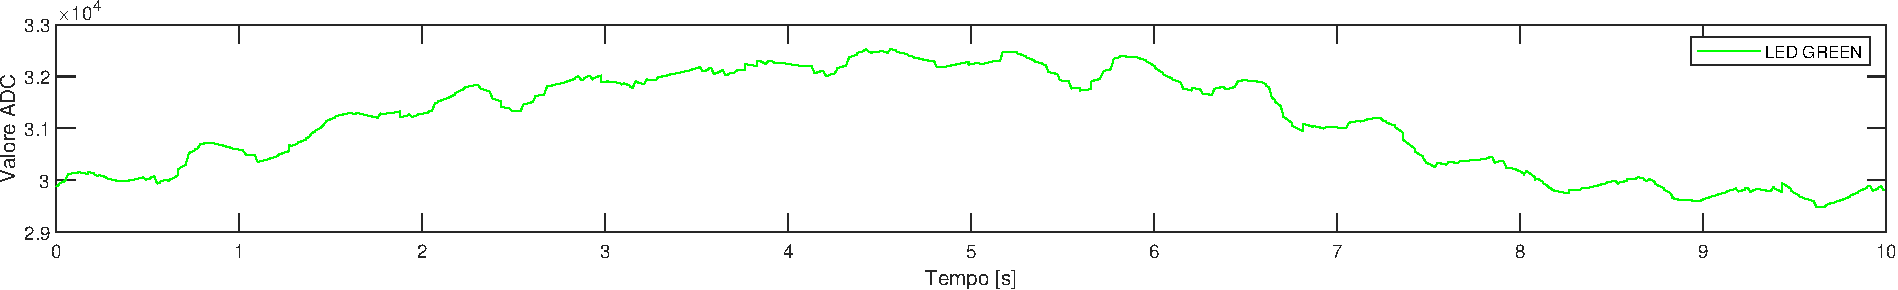
\includegraphics[width=1\linewidth]{ImageFiles/Misure Preliminari/Soggetto 1/polpastrello_green}
	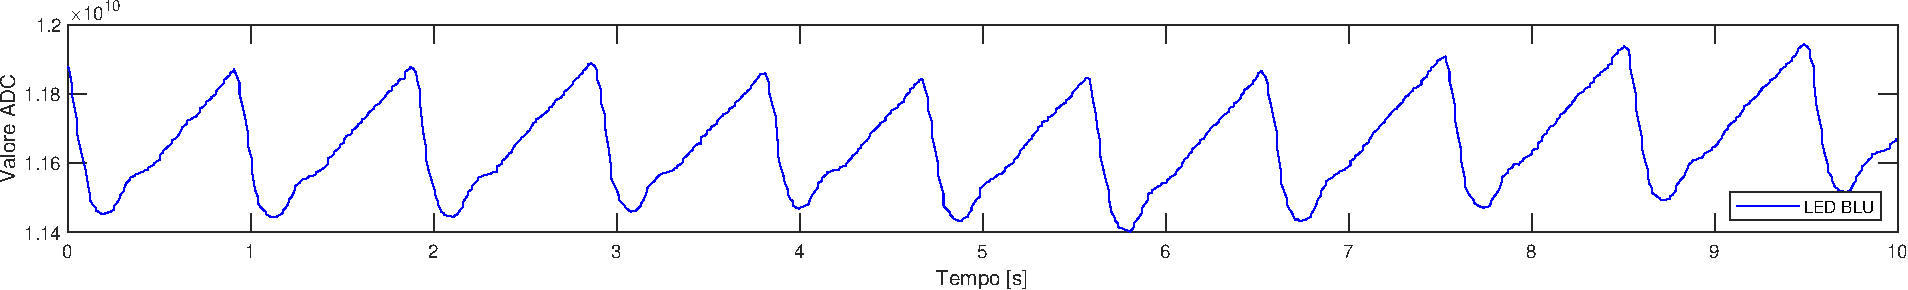
\includegraphics[width=1\linewidth]{ImageFiles/Misure Preliminari/Soggetto 1/polpastrello_blu}
	\caption{Segnali PPG acquisiti sul polpastrello del dito indice sinistro.}
	\label{fig:soggetto1_polpastrello}
\end{figure}
Il polpastrello rappresenta il sito di misura più utilizzato poiché permette di ottenere ottimi segnali PPG ed è facilmente indossabile. Come si può notare in figura \ref{fig:soggetto1_polpastrello}, tutte le misurazioni presentano una buona e distinguibile componente AC. Infatti, è possibile distinguere sia il picco sistolico sia il picco diastolico anche con la luce verde e blu. Le acquisizioni con la luce verde e blu presentano un andamento più \textit{smooth}. Questa caratteristica è determinata dalla minore penetrazione della luce verde-blu, che rende le misurazioni meno soggette ad interferenze dovute a movimenti, anche minimi, del soggetto. La figura rappresenta il segnale PPG nell'arco di 10 secondi. Contando i picchi presenti, e moltiplicandoli per un fattore 6, è possibile effettuare una stima della frequenza cardiaca del soggetto. In questa misurazione, si possono individuare 12 picchi, stimando una frequenza cardiaca di 72 battiti al minuto. La luce verde presenta una componente DC maggiore rispetto \todo{componente dc}

\paragraph{Lobo orecchio destro}
\begin{figure}[h]
	\centering
	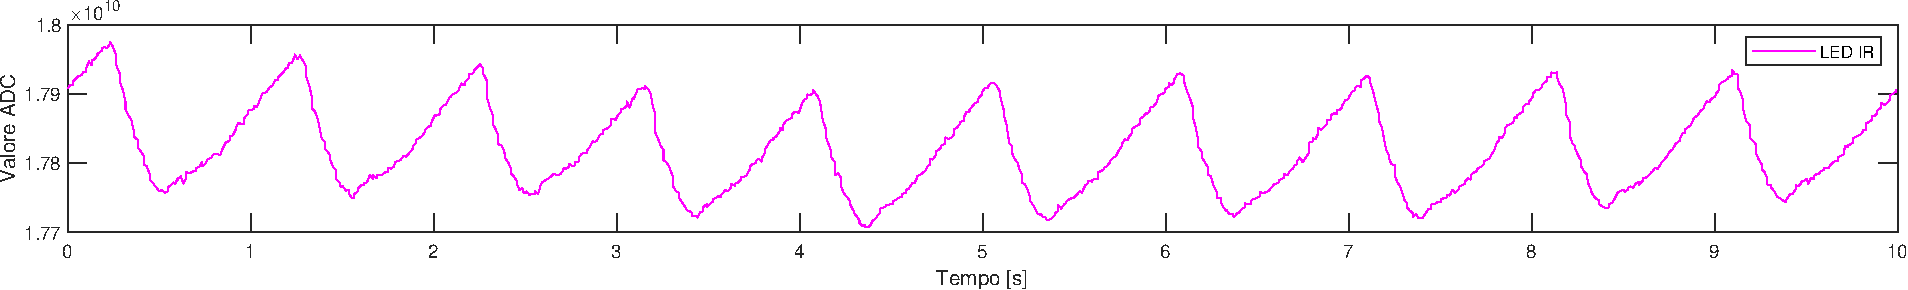
\includegraphics[width=1\linewidth]{ImageFiles/Misure Preliminari/Soggetto 1/lobo_ired}
	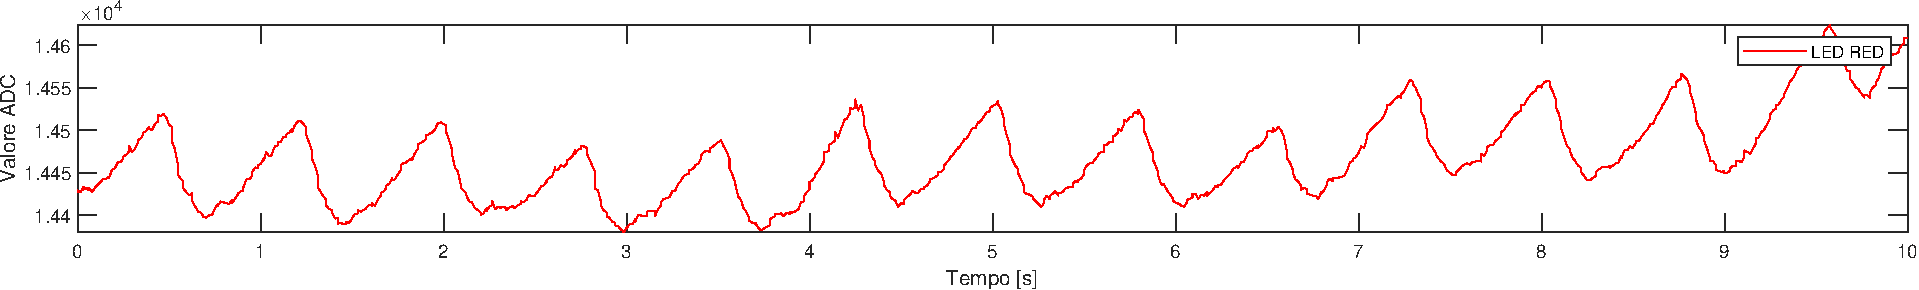
\includegraphics[width=1\linewidth]{ImageFiles/Misure Preliminari/Soggetto 1/lobo_red}
	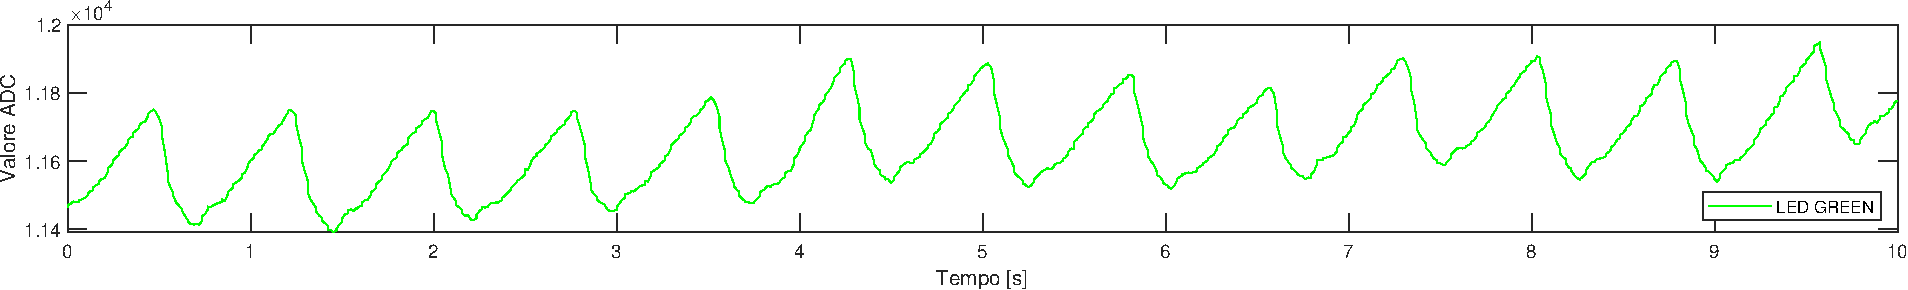
\includegraphics[width=1\linewidth]{ImageFiles/Misure Preliminari/Soggetto 1/lobo_green}
	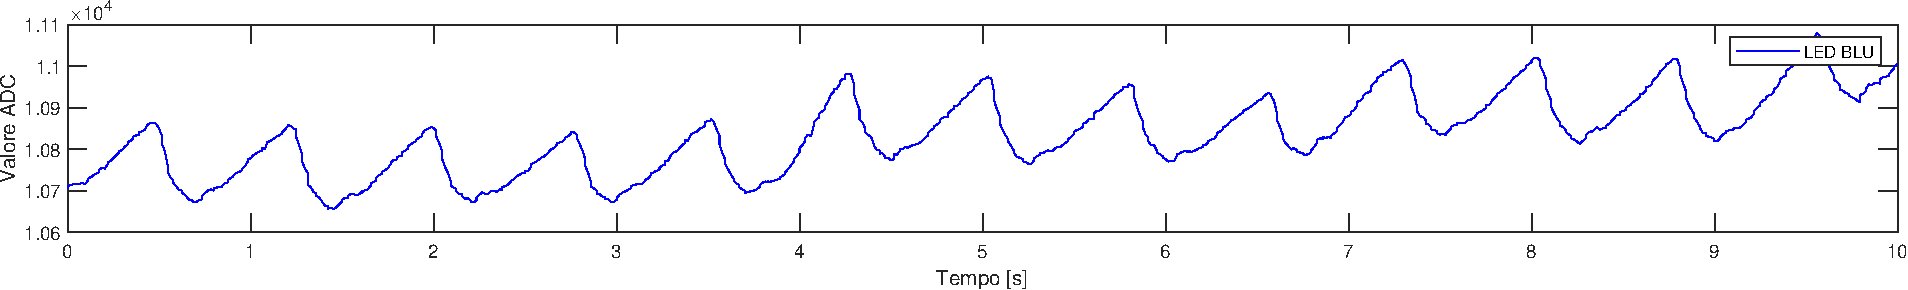
\includegraphics[width=1\linewidth]{ImageFiles/Misure Preliminari/Soggetto 1/lobo_blu}
	\caption{lobo}
	\label{fig:Descrizione_Segnale_PPG}
\end{figure}


\paragraph{Polso antero-interno}
\begin{figure}[h]
	\centering
	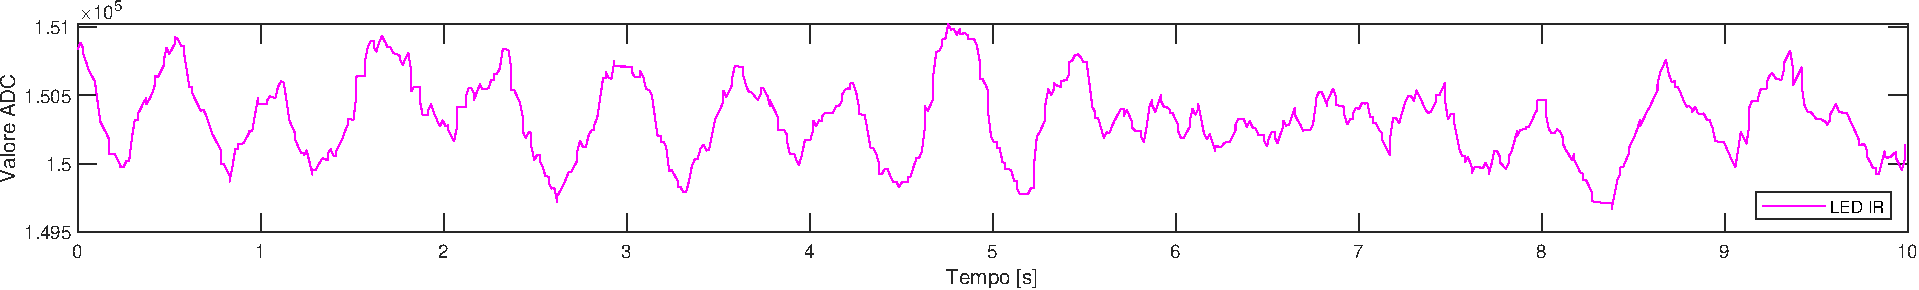
\includegraphics[width=1\linewidth]{ImageFiles/Misure Preliminari/Soggetto 1/polso_ired}
	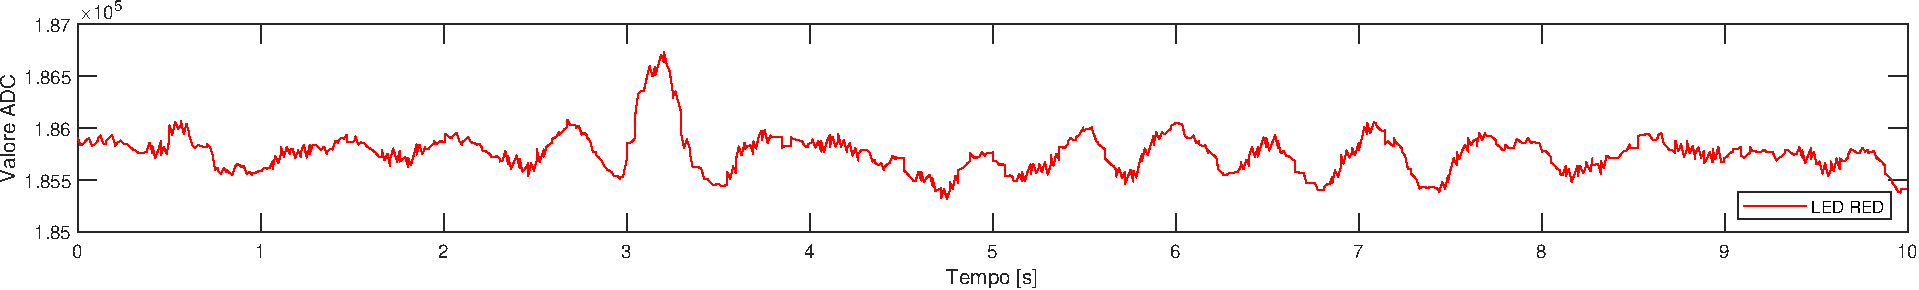
\includegraphics[width=1\linewidth]{ImageFiles/Misure Preliminari/Soggetto 1/polso_red}
	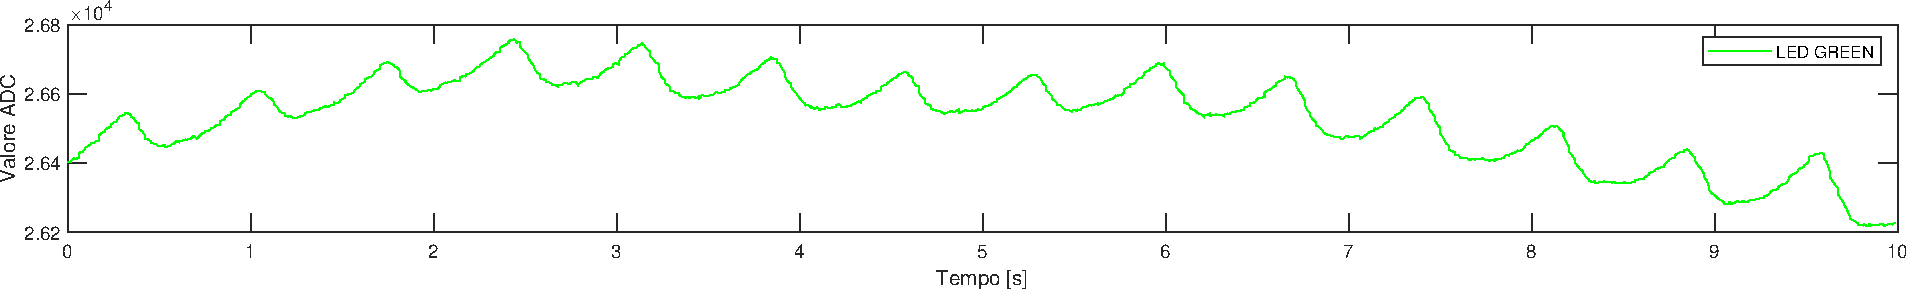
\includegraphics[width=1\linewidth]{ImageFiles/Misure Preliminari/Soggetto 1/polso_green}
	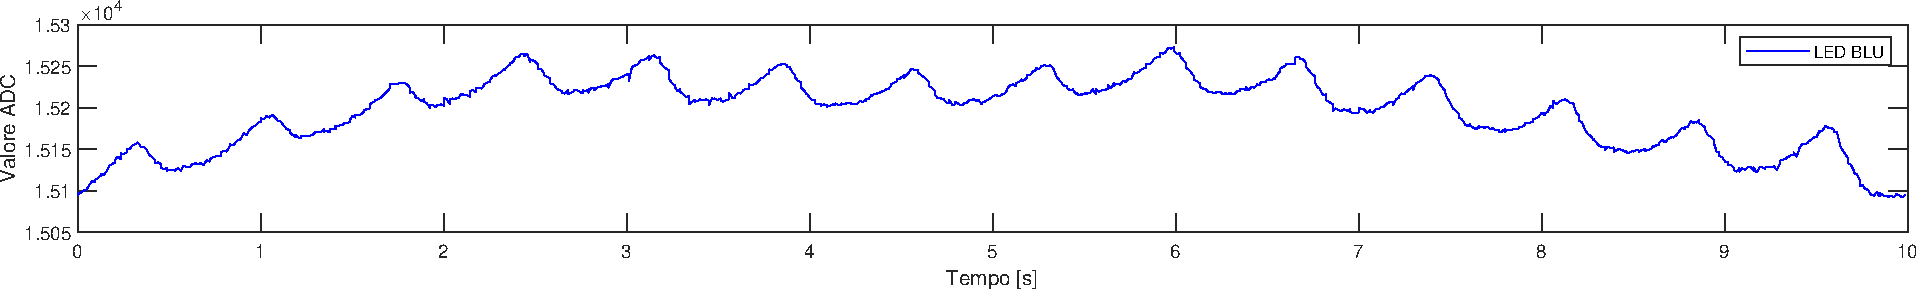
\includegraphics[width=1\linewidth]{ImageFiles/Misure Preliminari/Soggetto 1/polso_blu}
	\caption{polso}
	\label{fig:Descrizione_Segnale_PPG}
\end{figure}

\paragraph{Fronte}
\begin{figure}[h]
	\centering
	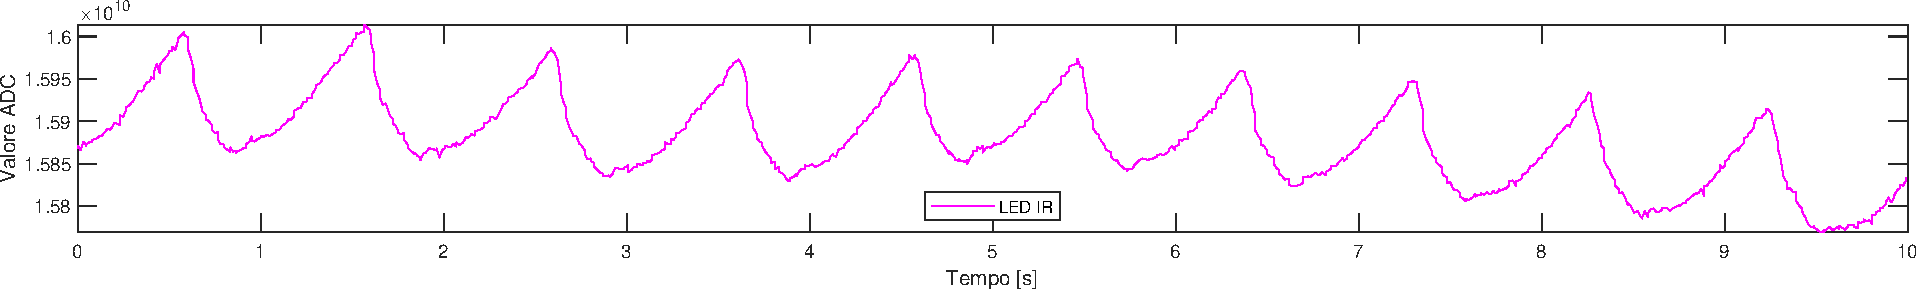
\includegraphics[width=1\linewidth]{ImageFiles/Misure Preliminari/Soggetto 1/fronte_ired}
	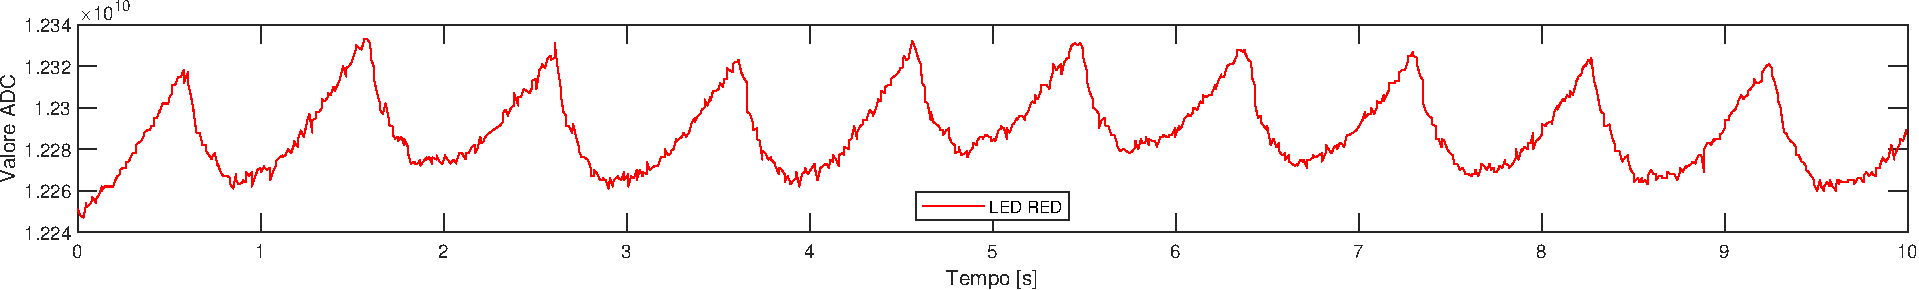
\includegraphics[width=1\linewidth]{ImageFiles/Misure Preliminari/Soggetto 1/fronte_red}
	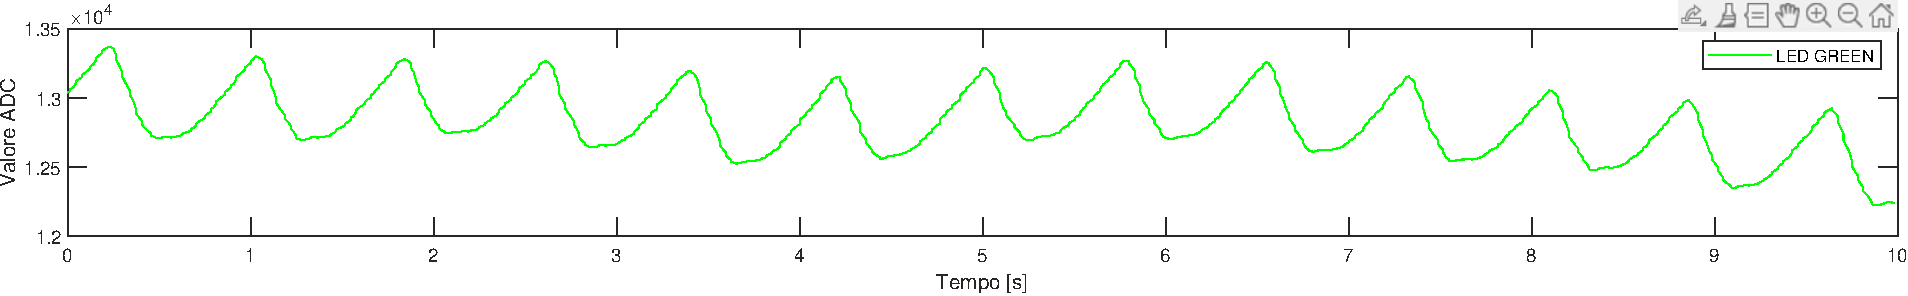
\includegraphics[width=1\linewidth]{ImageFiles/Misure Preliminari/Soggetto 1/fronte_green}
	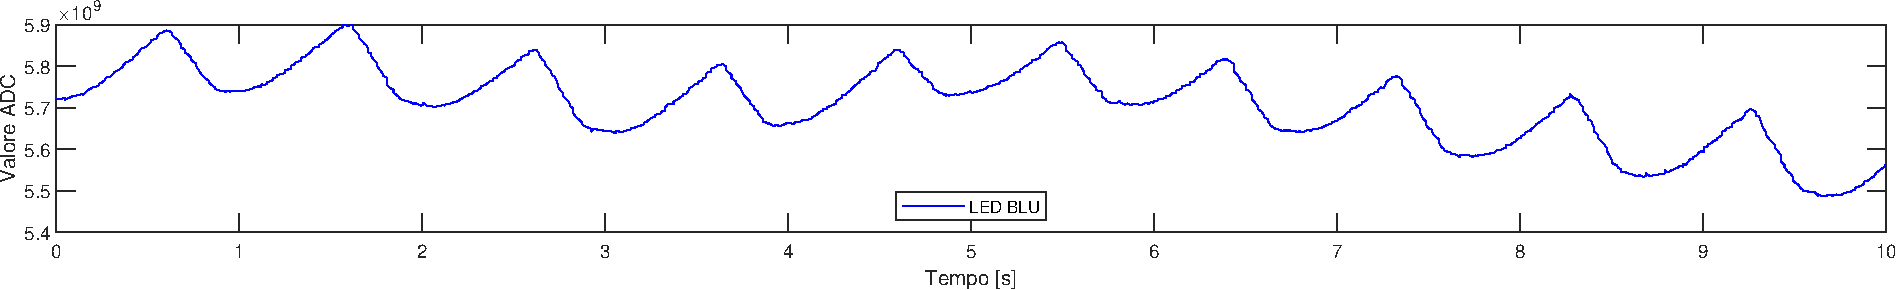
\includegraphics[width=1\linewidth]{ImageFiles/Misure Preliminari/Soggetto 1/fronte_blu}
	\caption{fronte}
	\label{fig:Descrizione_Segnale_PPG}
\end{figure}






\clearpage